This section breaks down our layer abstraction to another level of detail. Altogether, our system is divided into 3 different layers, Presentation Layer, Application Layer, Data Access Layer. Each of these layers are further divided into multiple subsystems. The Presentation Layer has Request, XML and Response. The Application Layer is divided into Java, Database Connection and Data Access Query whereas the Data Access Layer consists of Firebase, SQLite and Global Barcode Inventory. When an user opens the app, they will see the presentation layer consisting of text, buttons, forms, etc made using XML. When user makes some request like checking whether "India pale ale" is present in the inventory, this layer communicates with the application layer which formats a query and passes it to the data access layer. The data access layer then runs this query and returns the results (list of all beverage matching that style) to the application layer which then converts these results into appropriate format so that it can be displayed in the presentation layer. 

\begin{figure}[h!]
	\centering
 	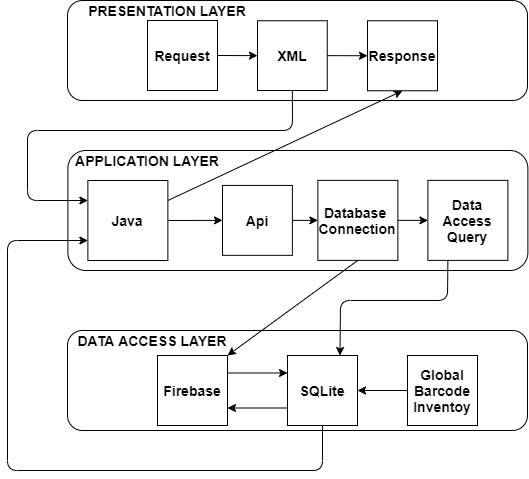
\includegraphics[width=\textwidth]{images/Full.png}
 \caption{A simple data flow diagram}
\end{figure}
